\documentclass[9pt]{extarticle}
\usepackage[T1]{fontenc}

%% Language and font encodings
\usepackage[english]{babel}
\usepackage[utf8x]{inputenc}

% table spacing
\usepackage{setspace}

%% zero set
\usepackage{amssymb}

%% Sets page size and margins
\usepackage[letterpaper,top=0.5cm,bottom=0.5cm,left=0.5cm,right=0.5cm,marginparwidth=0.25cm]{geometry}

%% Useful packages
\usepackage{amsmath}
\usepackage{graphicx}
\usepackage[colorinlistoftodos]{todonotes}
\usepackage[colorlinks=true, allcolors=blue]{hyperref}

% for compact, wrappable table
%\usepackage{showframe}% http://ctan.org/pkg/showframe
%\usepackage{booktabs}% http://ctan.org/pkg/booktabs
\usepackage{wrapfig,lipsum,booktabs}
\setlength{\textfloatsep}{0.1cm}

%% red bold text
\newcommand{\re}[1]{\textcolor{red}{\textbf{#1}}}

%% blue text
\newcommand{\bt}[1]{\textcolor{blue}{#1}}
%% blue normal text

%% pink bold text
\newcommand{\pute}[1]{\textcolor{pink}{\oldtextbf{#1}}}

\begin{document}
	\begin{wraptable}{l}{16cm}
		\begin{tabular}{c c c c c}
			 & \re{Distro} & \re{E(X)} & \re{V(X)} & \re{pmf} \\
			% \hline \\
			% BINOMIAL
			Binomial (discrete) &
			$X\mathtt{\sim}$Bin$(n,p)$ &
			$np$ &
			$np(1-p)$ &
			${n \choose x}p^{x}(1-p)^{n-x}$ \\
			% HYPERGEO
			Hypergeo (discrete) &
			$X\mathtt{\sim}$Hyper$(n,M,N)$ &
			$n\cdot\frac{M}{N}$ &
			\re{$\Big(\frac{N-n}{N-1}\Big)\cdot n \cdot \frac{M}{N}\cdot\Big(1 - \frac{M}{N}\Big)$} &
			\bt{$\frac{{M\choose x}{N-M \choose n-x}}{{N\choose n}}$} \\
			% NEGBIN
			NegBin (discrete) &
			$X\mathtt{\sim}$NegBin$(r,p)$ &
			$\frac{r(1-p)}{p}$ &
			$\frac{r(1-p)}{p^{2}}$ &
			${x+r-1 \choose r-1}p^{r}(1-p)^{x}$ \\
			% POISSON
			Poisson (discrete) &
			$X\mathtt{\sim}$Poi$(\mu)$ &
			$\mu$ &
			$\mu$ &
			\bt{$\frac{e^{-\mu}\cdot\mu^{x}}{x!}$} \\
			\hline
		\end{tabular}
	\end{wraptable}
	\noindent 
	\re{${n \choose k}$} $= \frac{n!}{r!(n-r)!} =$ ``n choose k''$=$ num combos of size $r$ that can be formed from $n$ indiv's in group
	\re{conditions for Bin} \bt{(1)} Two possible outcomes of each trial: S (what we counting) or
	F (all else). \bt{(2)} num trials $n$ is \emph{known and fixed} \bt{(3)} outcomes are
	\emph{independent} from one trial to others \bt{(4)} $p(\text{success})$ is \emph{same for all
	trials} \bt{(\textbf{$\cdot$})} if conditions met, $X={\text{num S's}}$ is binomial RV w/ params
	\re{n} number of trials / sample size and \re{p} probability of success.
	% CUT RANDOM INSIGHT INTO V(X)
	% \re{V(X)} of bin dist is largest (given $n$) when $p=0.5$ because \emph{the outcome is hardest to
	% predict!}
	% CUT BIN EXAMPLE 1
	%\re{ex1} suppose $p=0.7$. How does $P(X=x)$ change? Since $p(S)$ went up, more successful
	%outcomes; probabilities would shift towards largue values of $X$. Expect 2--3 S's to be most
	%likely X-val since $70\%$ of 3 is between (2,3).
	% CUT BIN EXAMPLE 2
	%\re{ex2} $10\%$ Americans left-handed. $X=$ num $\ell$-handed Americans in random sample of 12.
	%$X\mathtt{\sim}$Bin$(n,p)$ with $(n,p)=(12,0.1)$.
	%\bt{(i)} mean val $=\mu=E(X)=np=1.2$ expected
	%$\ell$-hand people in sample of 12.
	%\bt{(ii)} SD $=\sigma=\sqrt{V}=\sqrt{np(1-p)}=1.04$ $\ell$-hand
	%people. Roughly, poss vals X will be about 1.04 people from mean val of 1.2. 
	%\bt{(iii)} prob that sample contains at most 2 $\ell$-hand Americans is
	%$P(X\leq 2)=P(X=0)+\ldots+P(X=2)=0.889$, so $88.9\% $ chance of finding 2 or fewer $\ell$-hand
	%people in 12-American sample
	\re{conditions for HyperG} when sampling \emph{without replacement} from a small population
	(population not at least $10\times$ sample size).
	\bt{(1)} pop is finite, consists of \re{N} individuals/objects
	\bt{(2)} 2 kinds of indivs/objs: success (S), failure (F); \emph{and there are} \re{M}$<N$
	successes in population
	\bt{(3)} a sample of \re{n} individuals are \emph{randomly selected without replacement}
	\bt{(\textbf{$\cdot$})} if conditions met, $X={\text{num S's}}$ is hypergeom rv
	% OPTIONAL
	\re{pmf explained} numerator: num ways to have $x$ successes \& $n-x$ failues.
	Denominator: num ways to select a subset of $n$ indivs/objs out of group of $N$
	\re{Finite Pop Correction Factor$=$} $1-[\frac{n-1}{N-1}]$, second term is proportion of population
	included in sample.
	% OPTIONAL
	Since $<1$, hyperG has \emph{smaller V(X)} than bin.
	% Contract example (5.19)
	\re{conditions for NegBin}
	\bt{(1)} exp consists of \emph{potentially infinite num of indep Bernoulli trials}
	\bt{(2)} two poss outcomes for each trial: S, F
	\bt{(3)} probability of success \re{p} is \emph{same for all trials}
	\bt{(4)} exp continues until a total of \re{r} successes have been observed, where $r$ is fixed
	int $>0$
	\bt{(\textbf{$\cdot$})} if conditions met, $X={\text{num fails before $r$th success}}$ is
	negbin rv dist dependent on r,p
	\re{Geom dist} special case of NegBin where $r=1$
	% CONSIDER CUTTING 
	\re{$P(12\leq X\leq 28) =$} $P(11<X<29)=P(X=12)+\ldots+P(X=28)$
	\re{Continuous RVs} change: \emph{integration} instead of summation is now used to calculate
	probs, E's, V's. Also, \underline{CDF's} play more central role in finding probs,
	\emph{percentiles}
	\re{conditions for continuity} $X$ is continuous if
	\bt{(i)} $X$ can be any value in an intrvl,
	such as [0,1] or even (-$\infty$,$\infty$), or union of disjoint intrvls, \underline{AND}
	\bt{(ii)} $P(X=c)=0$ for any possible val of $c$---i.e., no indiv. val of $X$ has a positive
	probability
	\bt{\textbf{($\cdot$)}} CRV's often used to represent measurements
	\re{Probability Density Funciton (pdf)} $f(x)$ defines shape of a continuous distro. Needs to
	be integrated to find probabilities. Has prop that, for a crv $X$ has property that, for any two
	constants $a,b$:
	\re{$P(a\leq X\leq b)$} = $\int_{a}^{b}f(x)dx$
	\re{pdf criteria}
	\bt{(1)} $f(x)$ is \emph{non-negative}: $f(x)\geq 0$ for all -$\infty<x<\infty$
	\bt{(2)} entire area under $f(x)$ is 1: $\int_{-\infty}^{\infty}f(x)dx = 1$
	\re{P($X\leq 0.5$)} $= \int_{a}^{0.5}f(x)dx$
	\re{Uniform Dist}
	$f(x)=\frac{1}{b-a}$ for $a\leq x \leq b$, $0$ otherwise (issa square wave)
	\re{Cumulative Distribution Function (cdf)}: the cdf $F(x)$ of a crv $X$ is
	\re{$F(x)$} $=P(X\leq x) = \int_{-\infty}^{x}f(y)dy$
	\re{cdf of uniform dist} $F(x) = \int_{a}^{x}\frac{1}{b-a}dy = \frac{x-a}{b-a} \leftarrow$
	straight line w/ $F(a)=0,F(b)=1$ and slope $1/(b-a)$
	\re{CDF Propositions} if $X$ is a crv with pdf $f(x)$ and cdf $F(x)$, $a,b$ any two numbers
	s.t. $a<b$, then
	\bt{(1)} \re{$P(X>a)$} $= 1-F(a)$
	\bt{(2)} \re{$P(a\leq X\leq b)$} $=F(b) - F(a)$
	\bt{(3)} \re{$P(X=x)$} $=0$ for all values of $x$. Resultantly,
	\b{(3.i)} $P(A\leq X\leq b) = P(a<X\leq b) = P(a\leq X < b) = P(a<X<b)$
	\bt{(4)} $f(x)$ is the derivative of $F(X)$: $f(x) = \frac{dF(x)}{dx}$
	\re{Expected value of $X$, $\mu_{X}=E(X)=$} $\int_{x}x\cdot f(x)dx$
	\re{Expected value of function, $\mu_{h(X)}=E(h(x))=$} $\int_{x}h(x)\cdot f(x)dx$
	\re{Variance of X, $\sigma_{X}^{2}=$} $V(X) = \int_{x}(x-\mu)^{2}\cdot f(x)dx
												= E(X^{2}) - [E(X)]^{2}$
	\re{Standard Deviation of X, $\sigma_{X}=$} $\sqrt{V(X)}$
	% E(X) uniform dist, 6.50
	\re{Percentile} for any continuous rv $X$, and for values of $p$ $(0<p<1)$, the
	$(100p)^{th}$ percentile, $\eta(p)$, of dist $X$ is defined by
	\re{$p = F(\eta(p))=$} $\int_{-\infty}^{\eta(p)}f(y)dy$
	\re{notes on percentile} $\eta(p)$ is the val in the distribution of $X$ s.t.
	$100p\%$ of area under density curve lies to the left of $\eta(p)$ and
	$100(1-p)\%$ lies to the right of $\eta(p)$.
	\re{to find $p^{th}$ percentile of any dist:} set $p$ equal to the cdf and solve
	for $x$!
	\re{Median $\tilde\mu$ of $X$} for any crv $X$, the median is the \emph{$50^{th}$
	percentile} of the dist $X$, s.t. $\tilde\mu$ satisfies $0.5=F(\tilde\mu)$. Half
	of area under density curve lies to left of $\tilde\mu$, and half to right.
	\re{mean vs median} median is middle val, won't be affected by outlier values.
	However, mean \emph{will} be affected. If distribution is right-skewed,
	median $<$ mean; if left-skewed, mean $<$ median
	\re{Normal (Gaussian) Dist, $X\mathtt{\sim}$N$(\mu,\sigma^{2})$} most common family; many rv's have (approx) normal dist,
	and if they don't, ther mean often does. Most large-sampling statistic inference
	relies upon normal distribution.
	\re{Normal pdf} a crv $X$ has a normal distribution w/ parameters $\mu$ and $\sigma$
	(or $\mu$ and $\sigma^{2}$) if pdf of $X$ is
	\re{$f(\mu,\sigma)=$} $\frac{1}{\sqrt{2\pi}\sigma}e^{-(x-\mu)^{2}/(2\sigma^{2})}$
	\re{notes on normal dist}
	\bt{(1)} $x$ can take any vals $-\infty<x<\infty$
	\bt{(2)} $\mu$ (although fixed) can take any vals $-\infty<x<\infty$
	\bt{(2.1)} $\mu$ is the \emph{mean} of the normal dist; this controls center of
	distribution
	\bt{(3)} $\sigma$ can take any vals $\sigma>0$
	\bt{(3.1)} $\sigma$ is the \emph{standard deviation} of the normal dist
	($\sigma^{2}$ is the variance); this controls the spread/scale of the dist
	\bt{($\cdot$)} normal dist always has bell shape
	% sketching a normal dist 7.6
	\re{sketching a normal dist}
	\bt{(i)} curve is tallest at $\mu$, at center
	\bt{(ii)} 99.7$\%$ of dist is between $\mu-3\sigma$ and $\mu+3\sigma$. These are
	the approx. smallest and largest vals of $X$
	\bt{(iii)} changing $\mu$ shifts entire distribution
	\bt{(iv)} changing $\sigma$ controls how tall/flat dist is
	\re{standard score z$=$} $\frac{x-\mu}{\sigma}$ tells you how many \emph{standard
	deviations} a particular observation is from mean. Dist from mean relative to how
	much \emph{variation} there is. Follows a \emph{standard normal distribution}
	\re{standard normal distribution} a crv $Z$ is said to have a \emph{standard
	normal distribution} if \bt{$\mu=0$} and \bt{$\sigma=1$}:
	$Z\mathtt{\sim}$N$(0,1)$
	\re{pdf Z $=$} $f(z;0,1) = \frac{1}{\sqrt{2\pi}}e^{-z^{2}/2}$
	\re{cdf Z $\Phi(z)=$} $P(Z\leq z) = \int_{-\infty}^{z}f(y;0,1)dy$
	\re{can find probabilities by}
	\bt{(1)} integrating the pdf $f(x)$, so $P(a<X<b) = \int_{b}^{a}f(x)dx$
	\bt{(2)} plugging values into cdf $F(x)$, so $P(a<x<b)=F(b)-F(a)$
	\re{finding probabilities using a normal dist}
	\bt{(i)} integrals must be
	approximated; difficult before computers were available
	\bt{(ii)} lots of possible normal distributions
	\bt{(iii)} soluiton (then): ``standardize'' each normal dist using standard score;
	get probabilities from table
	\bt{(iv)} solution (now): computing power
	\re{two ways to calc probabilities for a normal dist:}
	\bt{(1)} use table A3 in appendix, which gives values for $\Phi(z)$
	\bt{(2)} use graphing calc
	\re{e.g.} for $Z\mathtt{\sim}$N$(0,1)$, P($Z < -1.37$) $=\Phi(-1.37)$, so nav to
	row $z=-1.3$ and col $z=0.07$ and it's there
	\re{for greater-thans:} table only gives CDF$=P(Z<z)$. To find $P(Z>z)$, need to
	subtract prob provided by table from 1
	\re{inequalities} $P(-2<Z<2) = \Phi(2) - \Phi(-2)$ (see \bt{pic 1, pic 3})
	% img here for wierder example 
	\re{calc} TI-83:
	$2^{nd}\rightarrow$VARS$\rightarrow$2:normalcdf(LB,UB,$\mu$,$\sigma$). if one of
	bounds is infinity, enter really big (/small) number. to find \bt{percentile} via
	calc, use invNorm func.
	\re{un-standardizing a table val} $x=z\cdot \sigma + \mu$
	\re{standardizing a probability} see \bt{pic 2, pic 4}
	\re{Normal approx. to Bin} $X\mathtt{\sim}$Bin$(n,p)$ can be written as
	$X=X_{1}+\ldots+X_{n}$
	\re{Central Limit Thm:} This $X$ is approximately normal or
	\re{$Z=\frac{X-np}{\sqrt{npq}}$} is approx standard normal $N(0,1)$ as
	$n\rightarrow\infty$. Good approx even if $n$ moderate ($\approx$30) and
	$np\geq5$ and $n(1-p)\geq 5$
	\re{Standardizing Normal Dists} if not standard normal dist, you'll have to
	standardize X val before using table
	\re{$B(n,p)\approx N(np,npq)$}
	\re{ex} $X\mathtt{\sim}$Bin$(n=15,p=0.4)$, $Y\mathtt{\sim}$N$(np,npq)=$N$(6,3.6)$
	then $P(X=5)\approx P(4.5<Y<5.5) =
	P(\frac{4.5-6}{\sqrt{3.6}} < P(\frac{Y-6}{\sqrt{3.6}}
							   < P(\frac{5.5-6}{\sqrt{3.6}})
							   		 = P(Z<-0.2635) - P(Z<-0.7906)
									 = 0.1815$, while exact $P(X=5)=0.1859$
	\re{Gamma function $\Gamma (\alpha)$}
	\bt{(1)} for any $\alpha>1$, $\Gamma (\alpha)
	= (\alpha - 1)\Gamma(\alpha - 1)$.
	\bt{(2)} For any positive int $n$, $\Gamma(n) = (n-1)!$
	\bt{(3)} $\Gamma(1/2) = \sqrt{(\pi)}$
	\re{Gamma Distribution $X\mathtt{\sim}$Gamma$(\alpha,\beta)$} \emph{not} the gamma
	function!!! Often used for \emph{waiting times} or \emph{survival times}
	\re{Gamma PDF} $f(x;\alpha,\beta)
					= \frac{x^{\alpha-1}e^{-x/\beta}}{\beta^{\alpha}\Gamma(\alpha)}$
	\re{Gamma CDF} $F\Big(\frac{x}{\beta}; \alpha\Big)
					 = \int_{0}^{x/\beta}\frac{y^{\alpha - 1}e^{-y}}{\Gamma(\alpha)}dy$
					 (probabilities found via a table)
	\re{Gamma E(X)} $=\alpha\beta$
	\re{Gamma V(X)} $=\sigma^{2}=\alpha\beta^{2}$
	\re{Gamma props}
	\bt{(1)} $x$ can only take non-neg vals: $x\geq 0$
	\bt{(2)} $\beta$ can only take pos vals: $\beta > 0$. $\beta$ is the \emph{scale}
	parameter; it controls \emph{spread} of dist. When $\beta=1$, $X$ is a
	\emph{standard} gamma dist: $f(x;\alpha)=\frac{x^{\alpha-1}e^{-x}}{\Gamma(\alpha)}$
	\re{Gamma prob} $P(X<6)=F(6/1;3)$ go to table A4, look for col $\alpha=3$ and down
	to row $X=6$. $P(2<X<5)=F(5/1;3)-F(2/1;3)$
	\re{Standardizing Gamma Dists} if $\beta\neq 1$, standardize X val before looking
	it up in table. e.g., for G(4,5), $P(X<8) = F(8/5;4) = F(1.6;4)$, make
	inequality: $F(1;4) < F(1.6;4) < F(2;4) \rightarrow 0.019 < P(X<8) < 0.143$
	\re{Special cases of Gamma dist}
	\bt{(i)} when $\alpha=1$ and $\beta>0$, gamma dist is
	the \bt{Exponential} dist w/ parameter $\beta$
	\bt{(ii)} when $\alpha=v/2$ and $\beta=2$, for pos int $v$, gamma dist is
	\emph{Chi-square} dist w/ param $v$---common dist for stat inference
	\re{Exponential Dist $X\mathtt{\sim}$Exp$(\lambda)$} special case of gamma dist.
	$x$ is non-neg, $\lambda$ is positive. Gen. skewed to right
	\re{Exponential PDF} $f(x;\lambda) = \lambda e^{-\lambda x}$
	\re{Exponential CDF} $F(x) = 1-e^{-\lambda x}$
	\re{Exponential $E(X)$} $= \frac{1}{\lambda}$
	\re{Exponential $V(X)$} $= \frac{1}{\lambda^{2}}$
	\re{hazard rate $\lambda$} higher value of $\lambda$ means shorter survival times.
	``Waiting time'' could also represent length of time between sucsesses of a
	\emph{Poisson} rv
	\re{notes Exp}
	\bt{(i)} sum of $\alpha$ pos independent Exp($\beta$) rv's can be modeled by
	the \bt{Gamma($\alpha, \beta$)} dist
	\bt{(ii)} exp dist is said to be \emph{memoryless}, i.e. $P(X>t+s/X>t)=P(X>s)$
	\bt{(iii)} gamma and other dists don't have this property
	\re{system of comopnents} each component lifetime $\mathtt{\sim}$Exp(0.01),
	component failures are independent, $A_{i}=$ith component lasts at least $t$ hours,
	and $X=$ time at which sys fails. Compute cdf $X$: $F(t) = P(X\leq t)$.
	Start by finding $P(X>t)$: $X>t \Leftrightarrow A_{1}\cap A_{2} \cap A_{3} \cap
	A_{4}$, so $P(X>t)=P(A_{1})\cdots P(A_{4}) = P(Y_{1}>t)\cdots P(Y_{4}>t)$ where
	$Y_{i}=$ lifetime of component $i$. Note cdf $Y_{i}$ is $P(Y_{i}\leq t)
	= (1 - e^{-0.01t})$, so $P(Y_{i} > t)$ is 1 minus that  $=e^{-0.01t}$. Then 
	$P(X>t) = e^{-0.04t} \Rightarrow F(t) = P(X\leq t) = 1 - e^{-0.04t}$, which is
	$X\mathtt{\sim}$Exp$(0.04)$
	\re{other exs} lifebulb follows exp dist; expected lifetime $1,000$ hrs.
	Prob rand-select bulb will last $>2,000$ hrs is, since we can get $\lambda=0.001$
	from $E(X)$, $P(X>2000) = 1 - F(2000;0.001) = e^{-(0.001)(2000)} = 0.135$ \\
	
	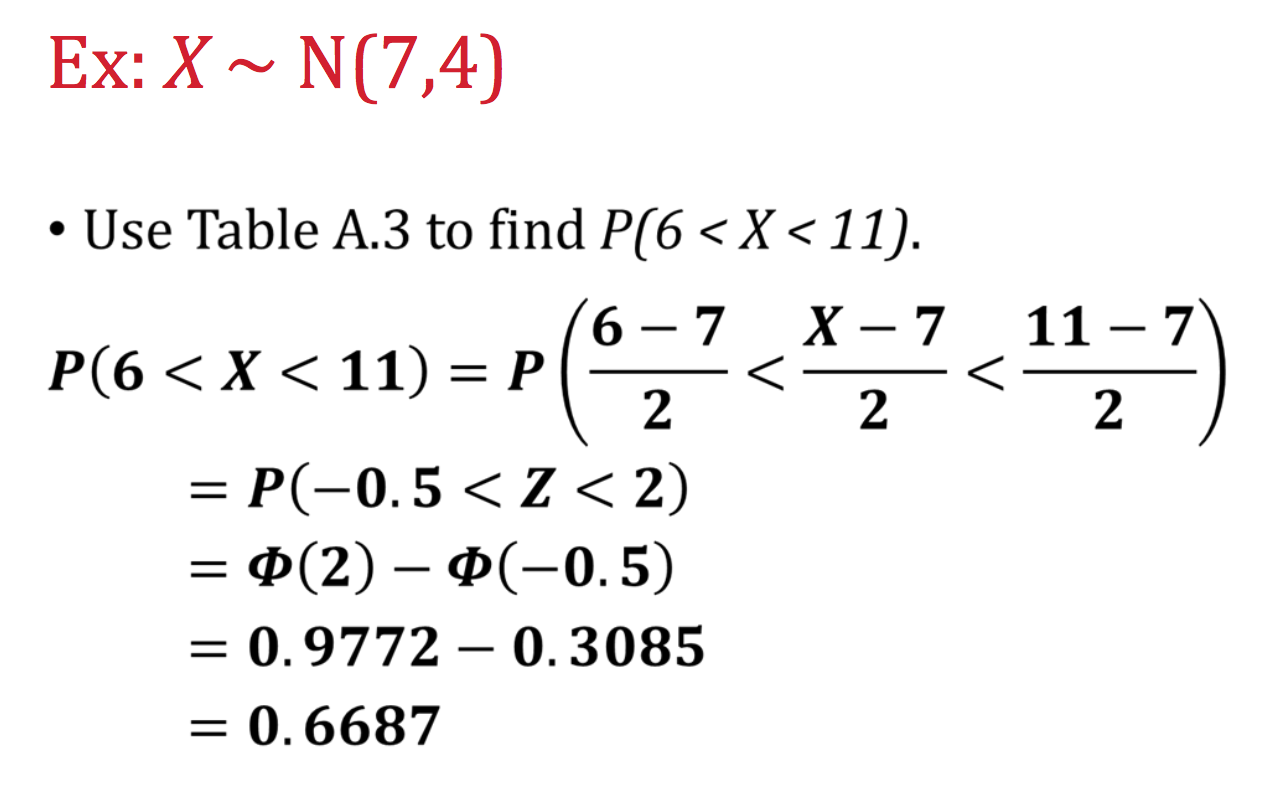
\includegraphics[scale=0.15]{1.png} 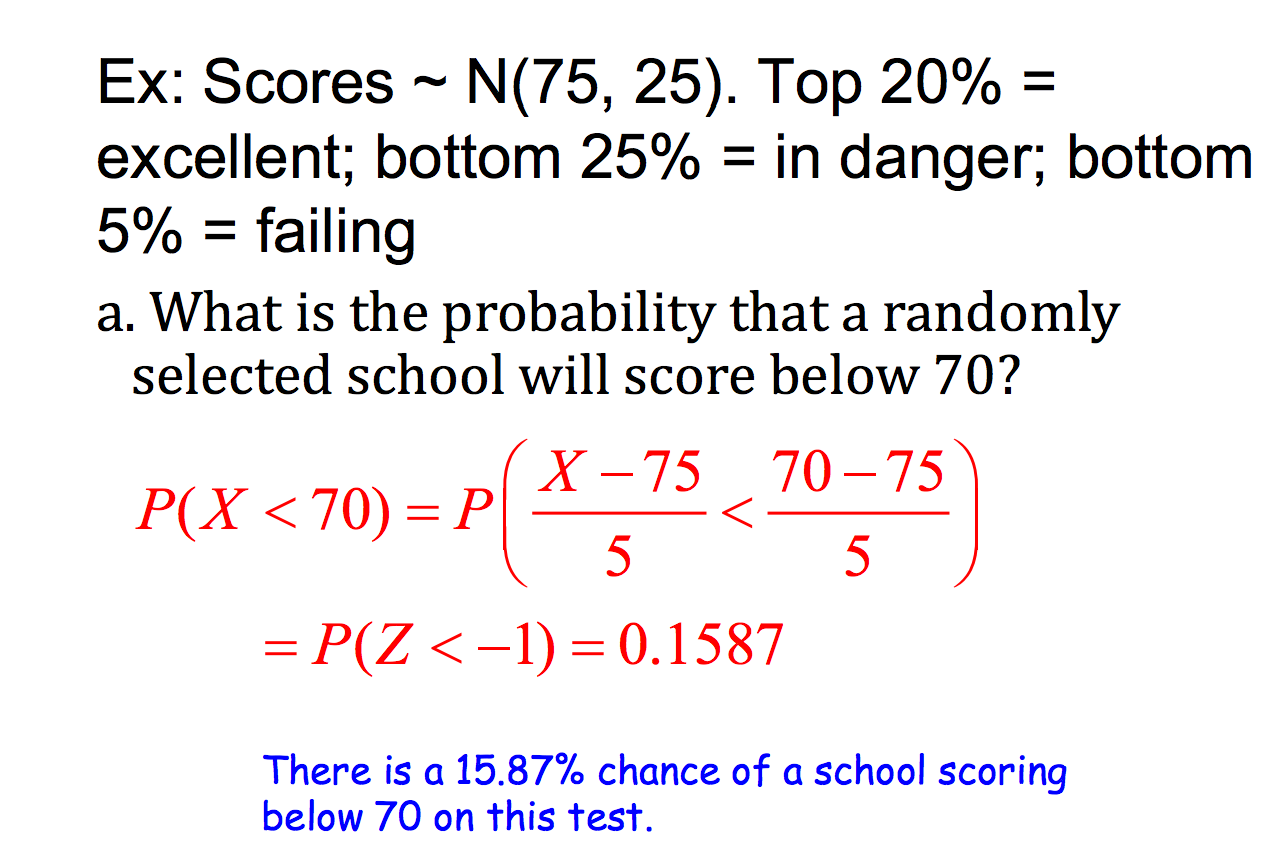
\includegraphics[scale=0.15]{2.png}
	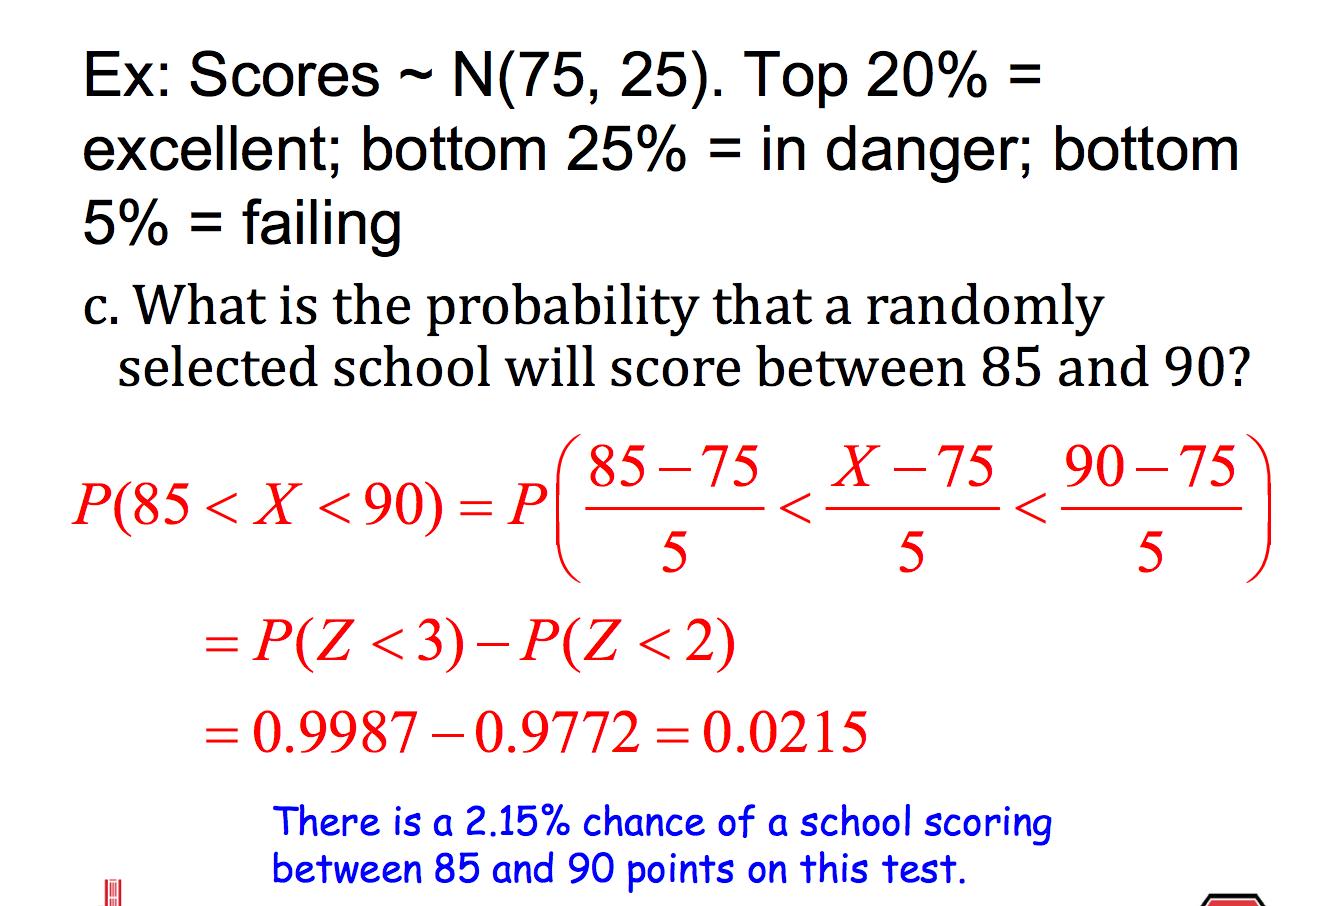
\includegraphics[scale=0.15]{3.png} 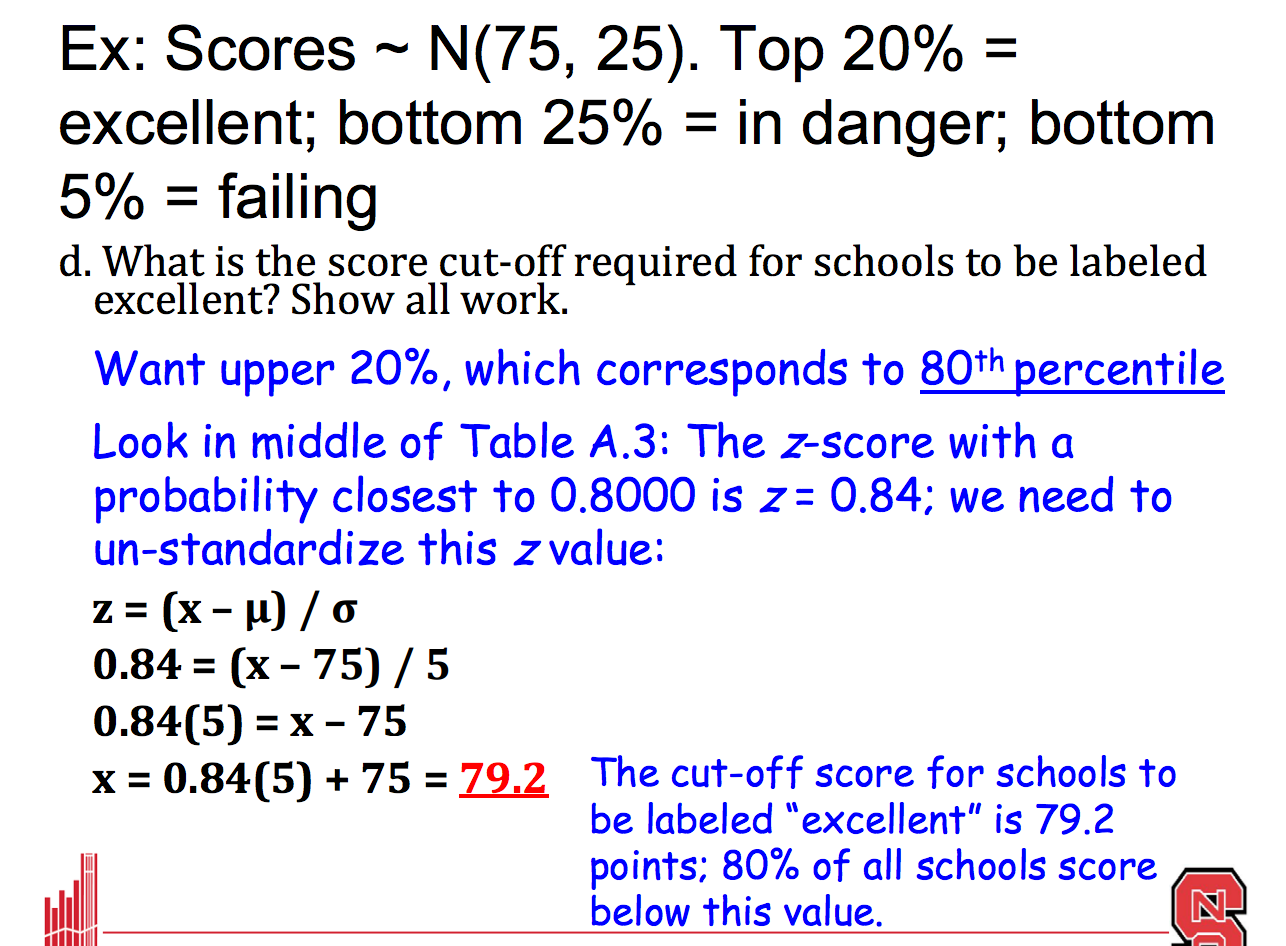
\includegraphics[scale=0.15]{4.png}
	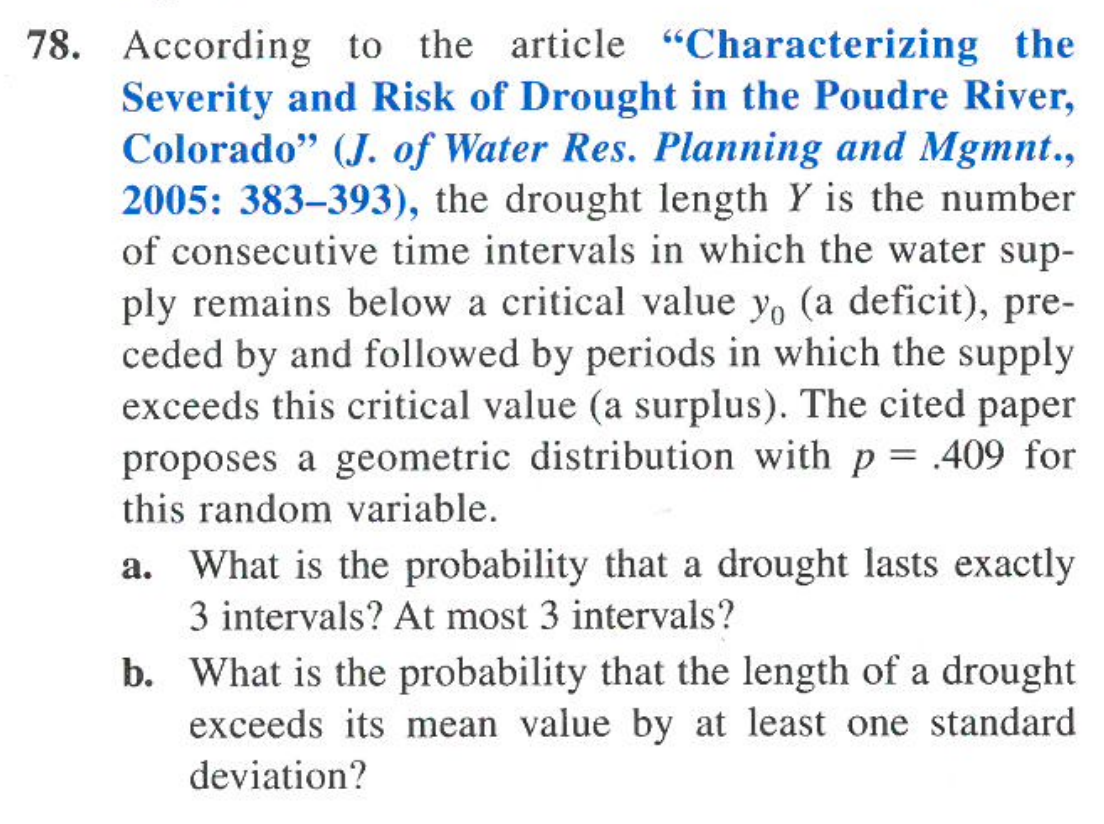
\includegraphics[scale=0.25]{78.png} 
	
	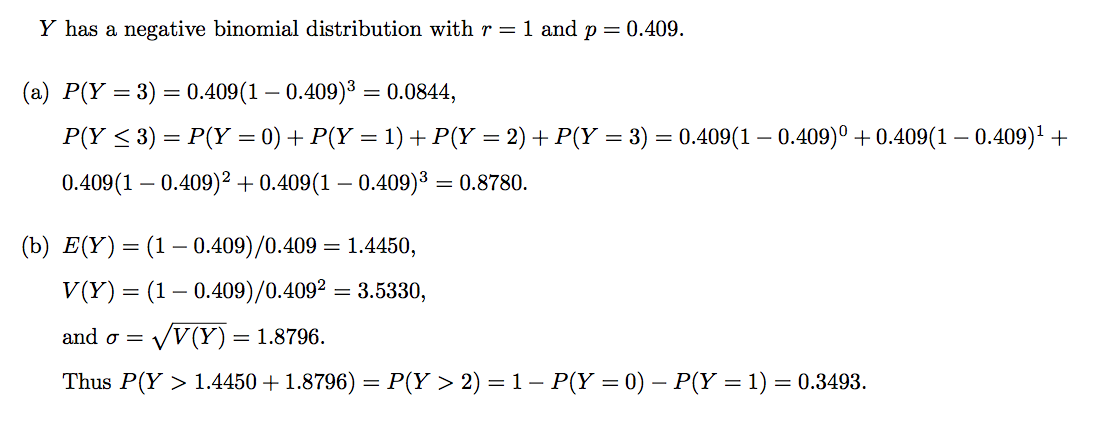
\includegraphics[scale=0.5]{78a.png} 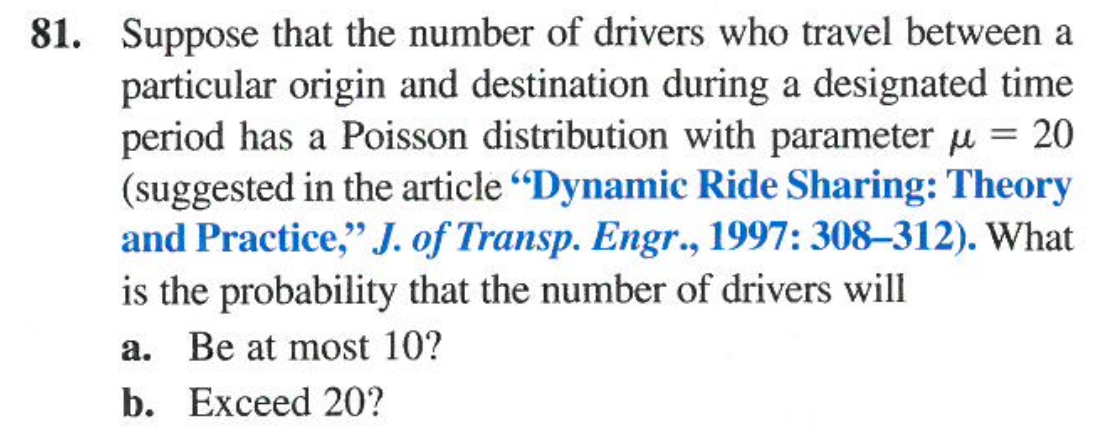
\includegraphics[scale=0.23]{81_1.png}
	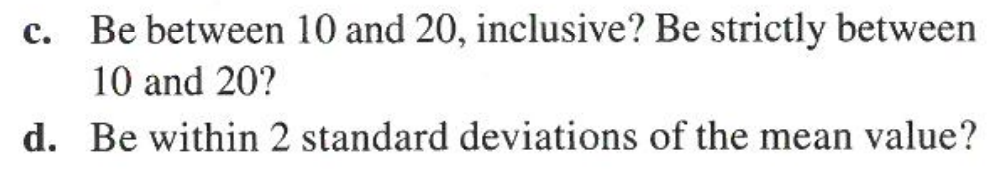
\includegraphics[scale=0.23]{81_2.png}
	
	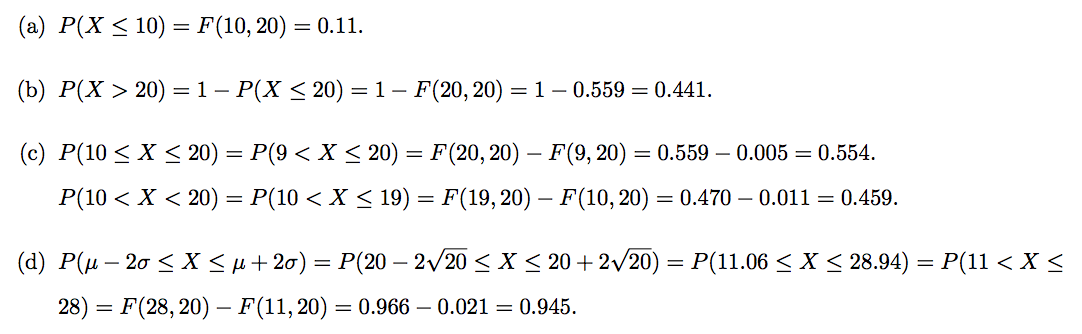
\includegraphics[scale=0.5]{81_a.png} 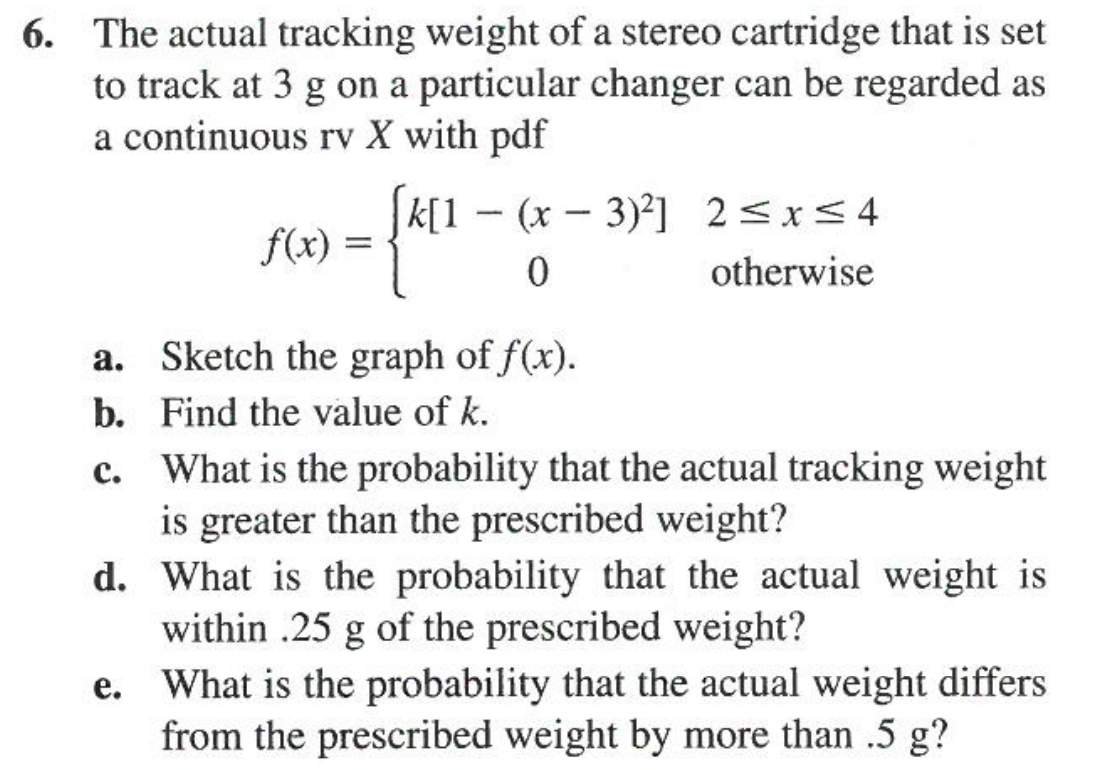
\includegraphics[scale=0.25]{6.png} 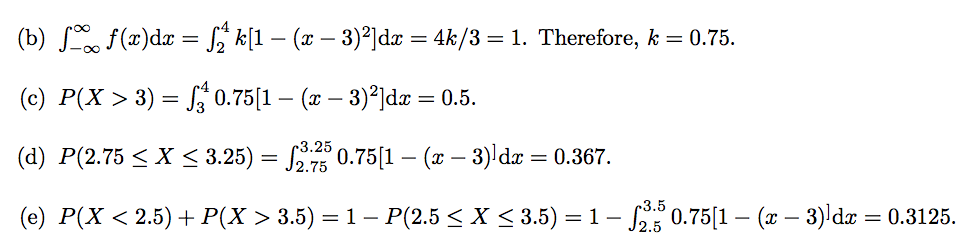
\includegraphics[scale=0.3]{6a.png}
	
	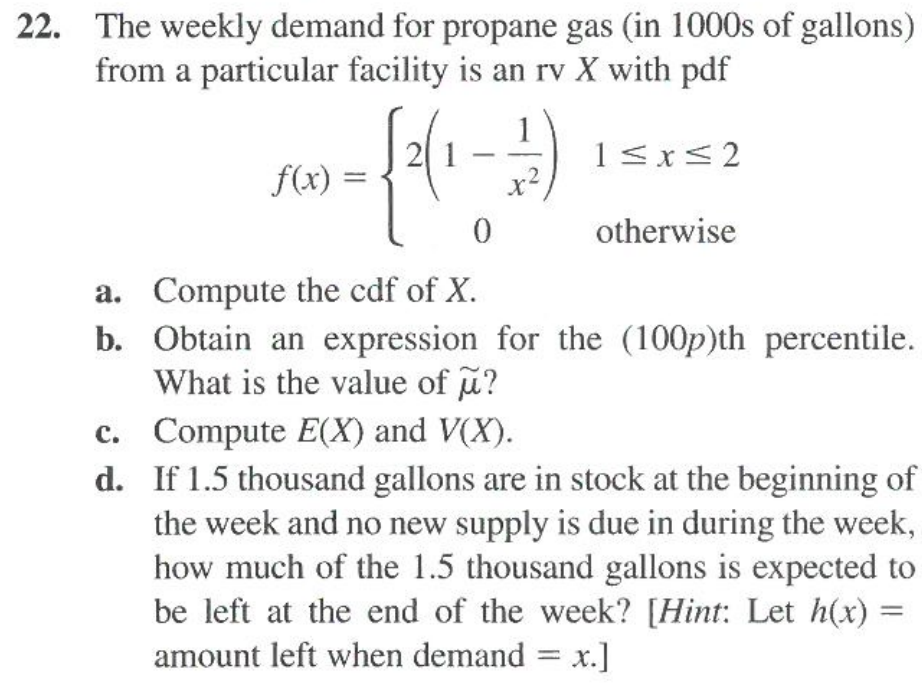
\includegraphics[scale=0.25]{22.png}
	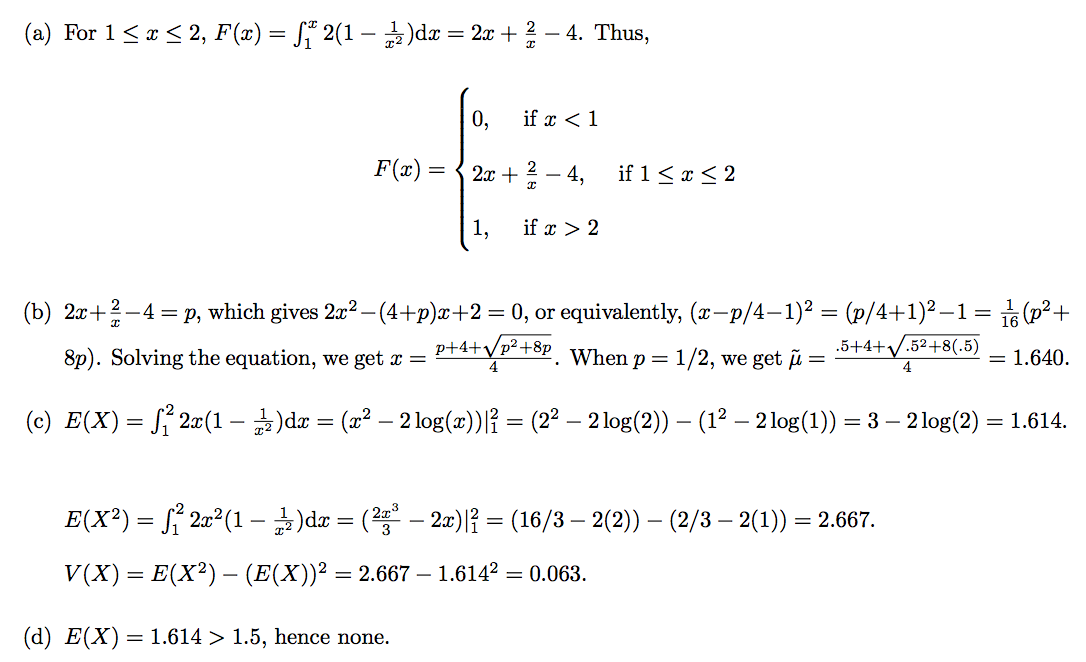
\includegraphics[scale=0.31]{22a.png} 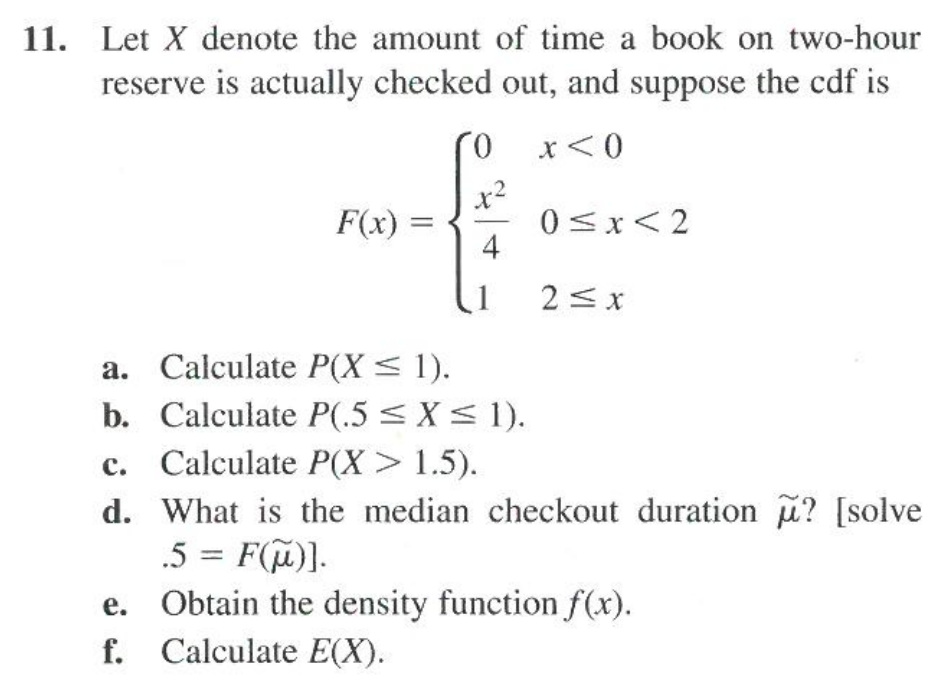
\includegraphics[scale=0.25]{11.png}
	
	 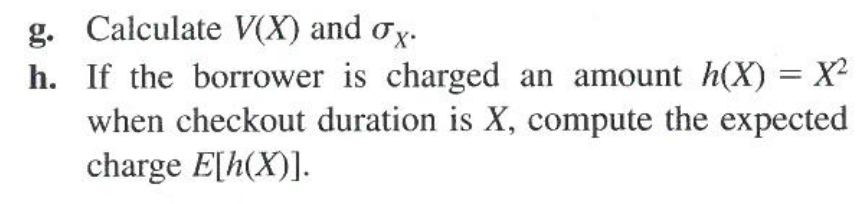
\includegraphics[scale=0.25]{11_2.png}
	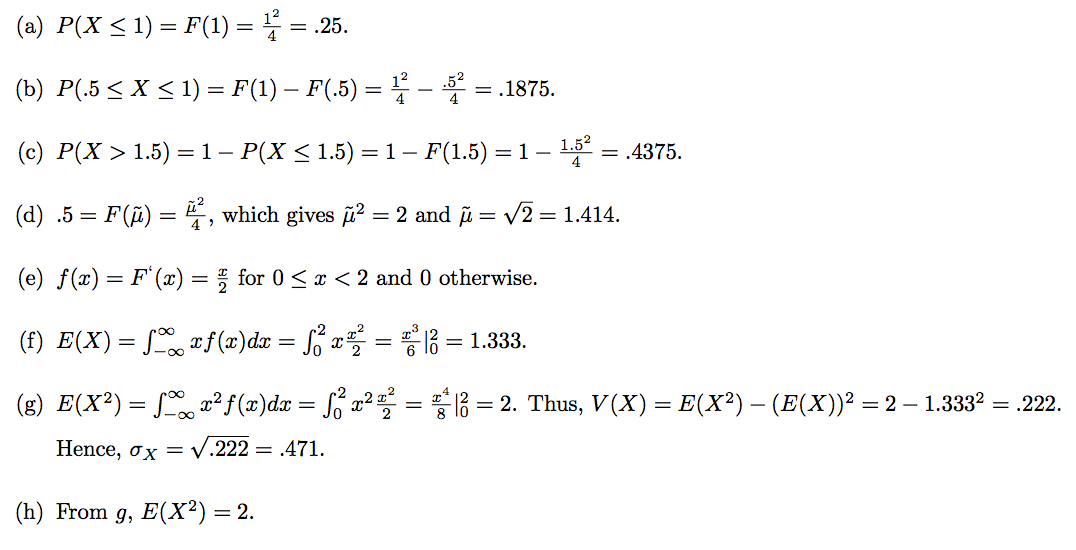
\includegraphics[scale=0.37]{11a.png} 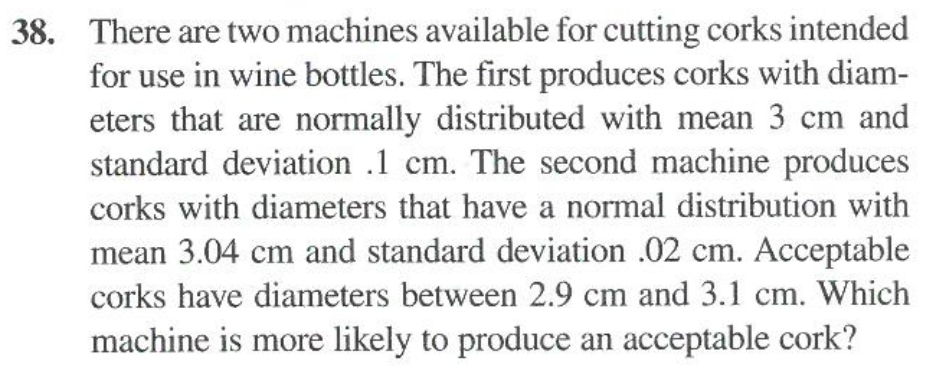
\includegraphics[scale=0.25]{31.png}
	
	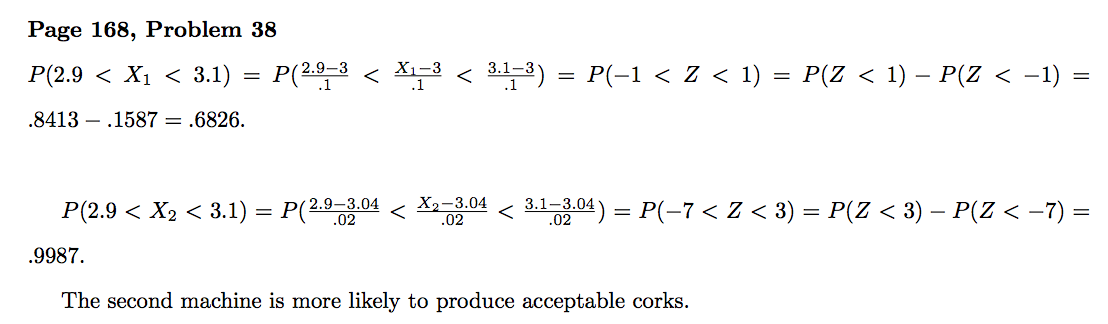
\includegraphics[scale=0.5]{31a.png}
	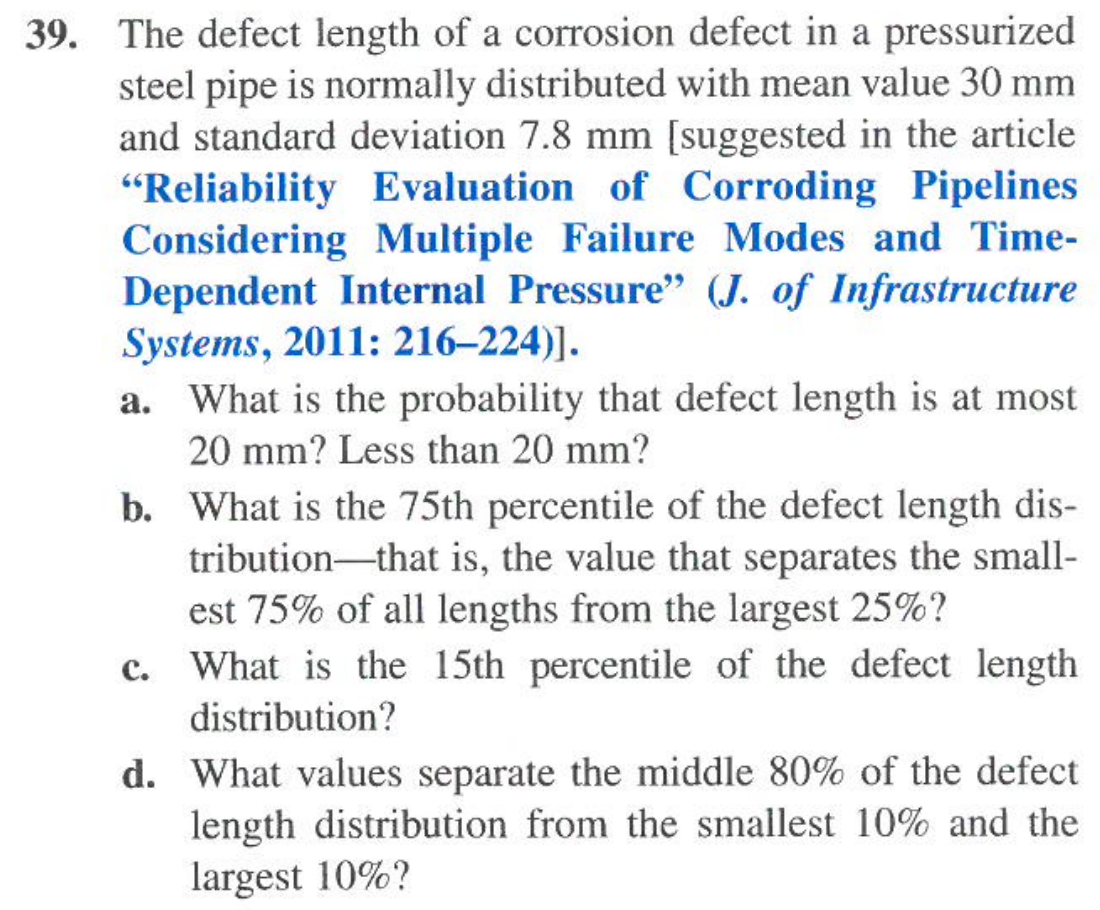
\includegraphics[scale=0.21]{39.png}
	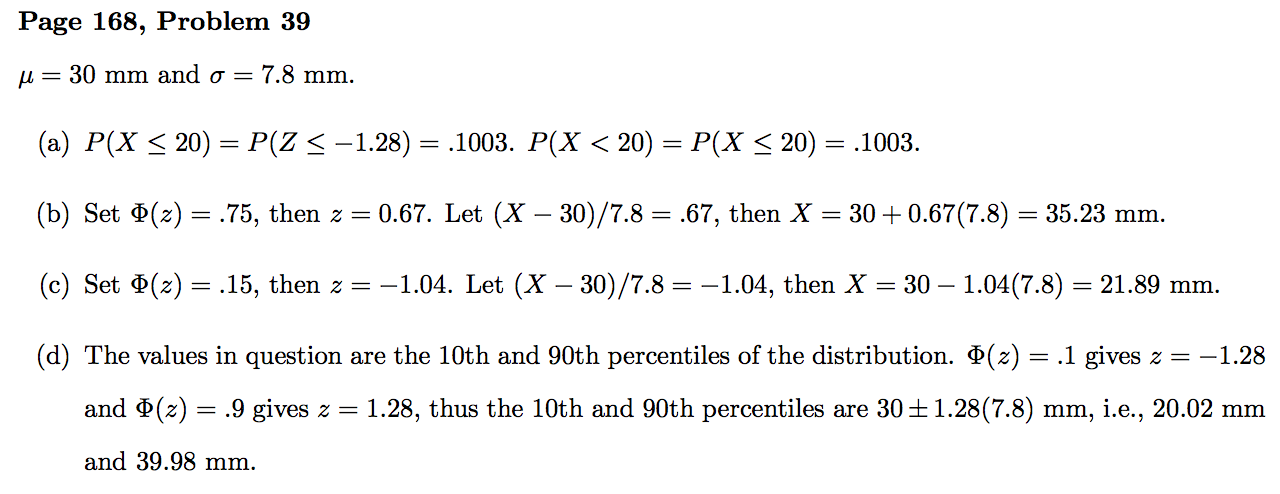
\includegraphics[scale=0.5]{39a.png}
	
	
	
	
	
	
	
	\pagebreak
	% SHORTCUTS
	\re{V(X)=} $E(X^{2})-(E(X))^{2}$
	\re{$\sigma =$}$\sqrt{V(X)}$
	
	
\end{document}